\section{Sequence Length and PIM Offload}
\label{sec:eval:seqlen}

The single-token results in Section~\ref{sec:eval:speedup} measure a workload
with little weight reuse. Each linear projection reads weights to process
one input vector. Prefill gives the CPU several tokens at once. It can reuse
fetched weights across these tokens through matrix--matrix multiplication.
This section examines how that changes the workload and whether the existing
\texttt{pim.gemv} path still helps.

The first experiment runs the GPT-3 layer on the CPU alone. It uses default
O3CPU, OpenBLAS and FP16 weights, as in the GPT-3 baseline. Decode processes one
new token with 256 tokens already in the KV cache. Prefill processes a prompt
of 4 to 512 tokens with an empty cache. Both use one input sequence. The
prefill program uses the same linear layers, but attention forms the full
score matrix and applies a causal mask.

\begin{figure}[htbp]
    \centering
    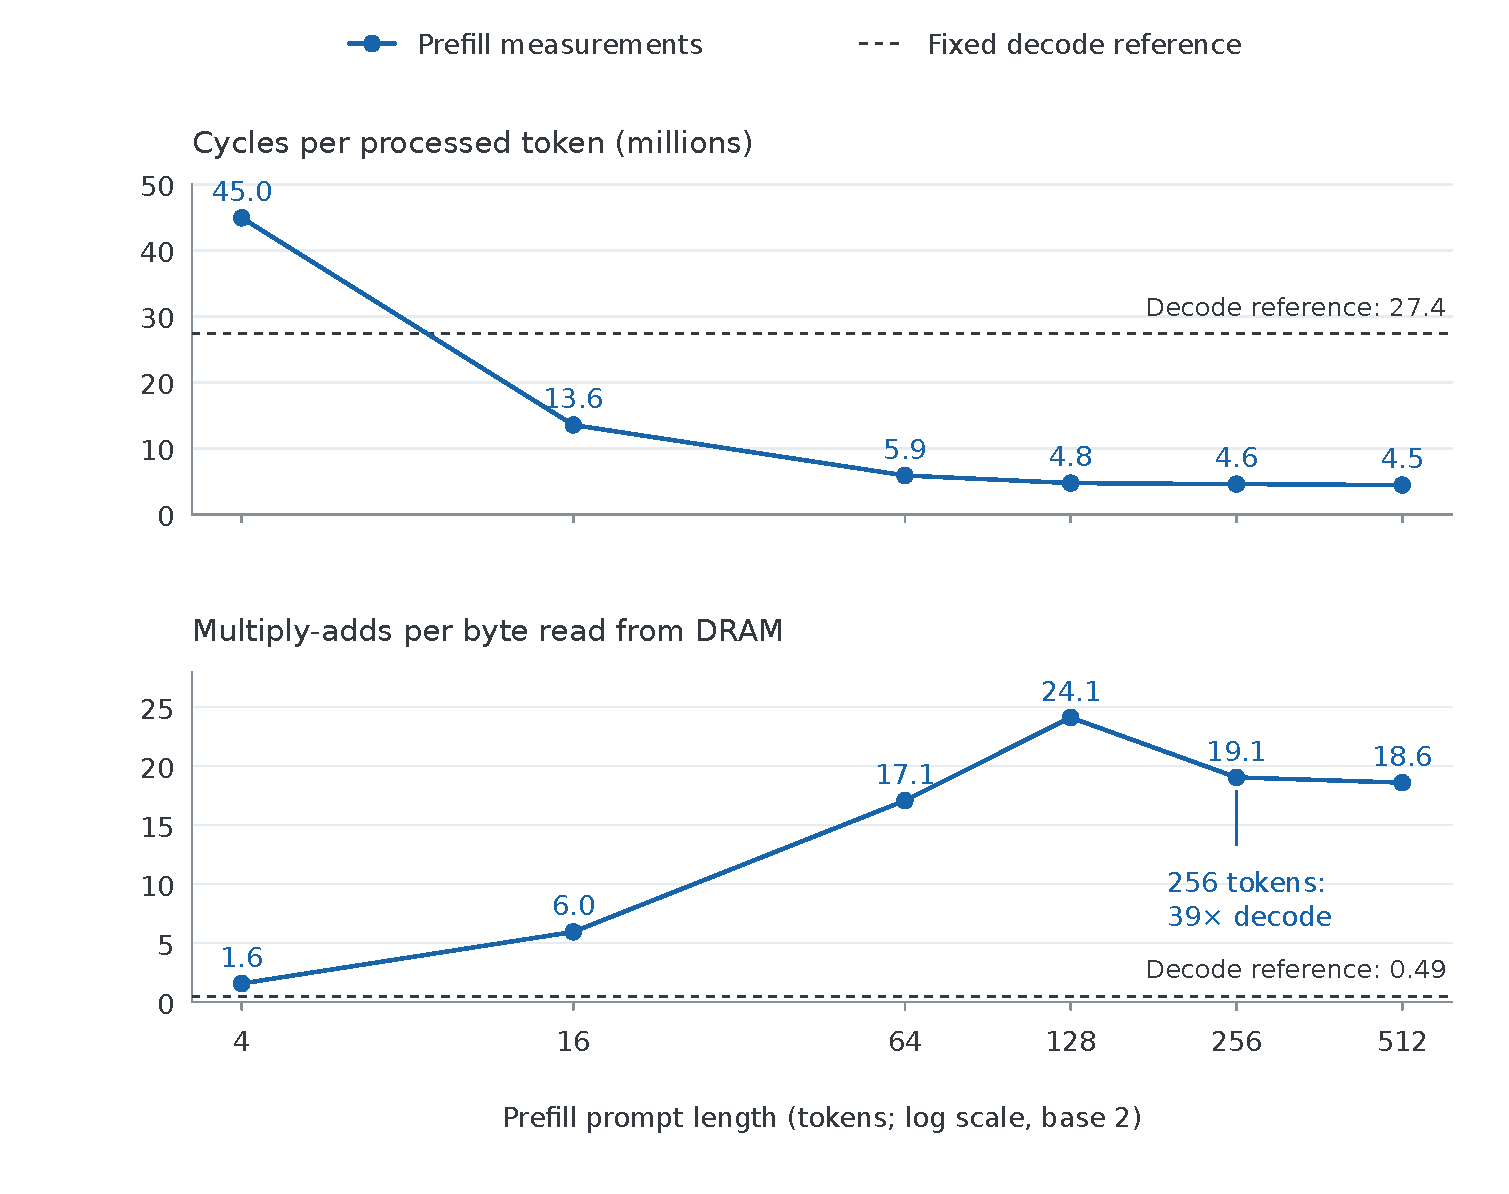
\includegraphics[width=\linewidth]{docs/diagrams/seqlen_performance.pdf}
    \caption{The CPU-only GPT-3 layer on default O3CPU with OpenBLAS and FP16
    weights, at batch size one. The upper panel shows cycles per processed
    token. The lower panel shows multiply-adds per byte read from DRAM.
    Solid curves show prefill with an initially empty KV cache. Dashed lines
    show one fixed decode reference: one new token with 256 cached tokens.
    Only prefill prompt length varies along the horizontal axis, which uses
    a logarithmic scale.}
    \label{fig:eval:seqlen}
\end{figure}

Figure~\ref{fig:eval:seqlen} shows the cost per token and the work done per
DRAM read byte. Decode takes 27.4 million cycles per token. Prefill takes
45.0 million at four tokens, 5.91 million at 64 tokens and 4.46 million at
512 tokens. Decode performs 0.49 multiply-adds per byte read from DRAM.
Its read bandwidth is 17.9~GB/s and its IPC is 0.50.
From 64 tokens onward, prefill performs
17 to 24 multiply-adds per read byte. This is 35 to 49 times the decode
value. Read bandwidth falls to between 2.1 and 2.9~GB/s, while IPC rises
to between 1.40 and 1.95. At 256 tokens, the prompt length
used by PIMony, multiply-adds per read byte are 39 times the decode value.
These results show more work per fetched byte. They do not, by themselves,
establish a point where PIM becomes slower than the CPU.

The ratio peaks at 128 tokens and then falls to about 19. Phase measurements
place the extra reads in the matrix multiplications. At 512 tokens,
$W_1$ reads 950~MB for a 52~MB weight matrix. Attention reads 98.5~MB.
The larger working set may interact with the 2~MiB L2 cache and OpenBLAS
blocking. The cause was not traced.

The CPU-only BERT runs show a similar pattern. At input lengths from 128
to 512 tokens, they perform 18 to 22 multiply-adds per read byte. Read
bandwidth is 1.1 to 1.3~GB/s and IPC is 1.5 to 1.8. These runs use FP32
weights. The BERT-sized results in Section~\ref{sec:eval:speedup} therefore
describe the single-token case. They do not measure full-sequence BERT
inference.

A separate experiment tests the PIM path directly on $W_1$, the feed-forward
projection from 2,560 to 10,240 values. It uses the same O3CPU and FP16 weight
precision. The CPU processes 64 input vectors together using OpenBLAS GEMM.
The PIM version processes the same vectors one at a time through the existing
offload path. Each vector requires three \texttt{pim.gemv} jobs. The PIM run
takes 0.486 million cycles per token, against 1.692 million on the CPU.
It is 3.48 times faster. The PIM time includes input staging, fences,
job issue, waiting and result readback. It measures the complete projection
offload, rather than the issue cost of one instruction.

The direct comparison shows that the current instructions still help this
projection at 64 tokens, despite the CPU's weight reuse. It does not measure
a complete prefill layer or locate a sequence length where PIM stops helping.
